\renewcommand{\theequation}{\theenumi}
\begin{enumerate}[label=\thesection.\arabic*.,ref=\thesection.\theenumi]
\numberwithin{equation}{enumi}
\item 
Find the equation of all lines having slope 2 and being tangent to the curve 
%\cite{twelve_one}
\begin{align}
\label{eq:hyperbola}
y + \frac{2}{x-3} = 0
\end{align}
\solution 
\eqref{eq:hyperbola} can be expressed as
\begin{align}
\label{eq:conic_nofrac}
xy -3y + 2 = 0
\end{align}
which is of the same form as \eqref{eq:conic_quad_form} with 
\begin{align}
\label{eq:hyper_quad_form_param}
\vec{V} = \frac{1}{2}\myvec{0 & 1\\ 1 & 0}, \vec{u} = -\frac{3}{2}\myvec{0 \\1}, f = 2
\end{align}
Using the approach in Example \ref{ex:ellipse_tangent},
\begin{align}
\vec{D} = \myvec{\frac{1}{2} & 0 \\ 0 & -\frac{1}{2}}, \vec{P} = \frac{1}{\sqrt{2}}\myvec{1 & -1\\1 & 1}
\end{align}
\begin{align}
\because \vec{u}^T\vec{V}^{-1}\vec{u}-f = -2 < 0,
\end{align} 
the major and minor axis are swapped and from Table \ref{table:conics}
the hyperbola parameters are given by 
\begin{align}
\vec{c}= 3\myvec{1\\0},
\sqrt{\frac{\vec{u}^T\vec{V}^{-1}\vec{u}-f}{\lambda_2}} = 2,
\\
\sqrt{\frac{f-\vec{u}^T\vec{V}^{-1}\vec{u}}{\lambda_1}} = 2
\end{align}
with the standard hyperbola equation becoming
\begin{align}
\frac{y_2^2}{4}-\frac{y_1^2}{4} = 1,
\label{eq:std_hyper}
\end{align}
%
Fig. \ref{fig:hyper_tangent}	shows  the actual hyperbola in \eqref{eq:hyperbola}  obtained from  
\eqref{eq:std_hyper}  using \eqref{eq:conic_affine}.  
The direction and normal vectors of the tangent with slope 2 are given by \eqref{eq:dir_vec_slope} and \eqref{eq:line_dir_norm} as
\begin{align}
\vec{m} = \myvec{1\\2}, \vec{n} = \myvec{2\\-1}
\end{align}
%
From \eqref{eq:conic_tangent_qk} and \eqref{eq:circle_tangent_prob_uf}, using \eqref{eq:hyper_quad_form_param},
\begin{align}
\kappa = \frac{1}{2}, \vec{q}_1 = \myvec{2\\2}, \vec{q}_2 = \myvec{4\\-2}.
\end{align}
%
The desired tangents are
\begin{align}
\myvec{2 & -1}\cbrak{\vec{x}-\myvec{2\\2}} &= 0 \implies \myvec{2 & -1} \vec{x} = 2
\\
\myvec{2 & -1}\cbrak{\vec{x}-\myvec{4\\-2}} &= 0 \implies \myvec{2 & -1} \vec{x} = 10
\end{align}
All the above results are verified in Fig. \ref{fig:hyper_tangent}.  As we can see, the hyperbola in \eqref{eq:hyperbola} is obtained by rotating the standard hyperbola by $\vec{P}$	and then translating it by $\vec{c}$.

\begin{figure}[!ht]
\centering
\includegraphics[width=\columnwidth]{./figs/hyper/hyper_tangent.eps}
\caption{Standard and actual hyperbola.}
\label{fig:hyper_tangent}	
\end{figure}

\end{enumerate}
